%%----------------------------------------------------------------------------
%% Presentatie HoGent Bedrijf en Organisatie
%%----------------------------------------------------------------------------
%% Auteur: Pieter Van Eeckhout [vaneeckhout.pieter@gmail.com]

\documentclass{beamer}

%==============================================================================
% Aanloop
%==============================================================================

%---------- Packages ----------------------------------------------------------
\usepackage{graphicx,multicol}
\usepackage{comment,enumerate,hyperref}
\usepackage{amsmath,amsfonts,amssymb}
\usepackage{tikz}
\usepackage[dutch]{babel}
\usepackage[utf8]{inputenc}
\usepackage{multirow}
\usepackage{eurosym}
\usepackage{listings}

%---------- Configuratie ------------------------------------------------------

\usetikzlibrary{arrows,shapes,backgrounds,positioning,shadows}

\usetheme{hogent}

%---------- Commando-definities -----------------------------------------------
\newcommand{\partTOC}{%
  \begin{frame}{overzicht}%
  \tableofcontents[currentpart]%
  \end{frame}%
}

%---------- Info over de presentatie ------------------------------------------

\title[Bachelorproef presentatie]{Oplossen van CAPTCHA testen gebruik makend van neurale netwerken}
\author{Pieter {Van Eeckhout} \small(stamnummer: 200901295)}
\date{\today}

%==============================================================================
% Inhoud presentatie
%==============================================================================

\begin{document}

%---------- Front matter ------------------------------------------------------

% Dia met het HoGent logo
\HoGentLogo 

% Titeldia met faculteitslogo
\begin{frame}[plain]
  \titlepage
\end{frame}

%---------- Inhoud ------------------------------------------------------------

% Dia voor sectiekop, voorbeeld met een afbeelding onderaan de pagina
\part{Situering}
\partframe{%
  \vfill%
  
\includegraphics[width=3cm]{logo/HG-woordmerk-inv}%
}
\part{Onderzoek}
\partframe{%
  \vfill%
  
\includegraphics[width=3cm]{logo/HG-woordmerk-inv}%
}
\partTOC
\section{CAPTCHA}
\subsection{Types}
\begin{frame}
\frametitle{Types CAPTCHA}
   \begin{columns}[c]
     \column{.30\textwidth}
       \begin{itemize}
  	     \item<+-> letter
  	     \item<+-> afbeelding
  	     \item<+-> afwijking
  	     \item<+-> herkenning
  	     \item<+-> geluid
       \end{itemize}
     \column{.70\textwidth}
       \begin{center}
         \only<1>{
\includegraphics[width=\textwidth]{./img/CAPTCHAtypes/letterCAPTCHA.png}}
         \only<2>{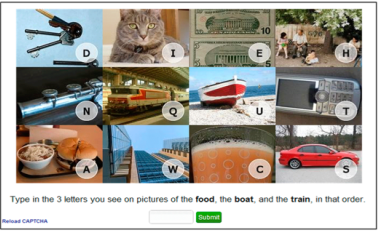
\includegraphics[width=\textwidth]{./img/CAPTCHAtypes/afbeeldingCAPTCHA.png}}
         \only<3>{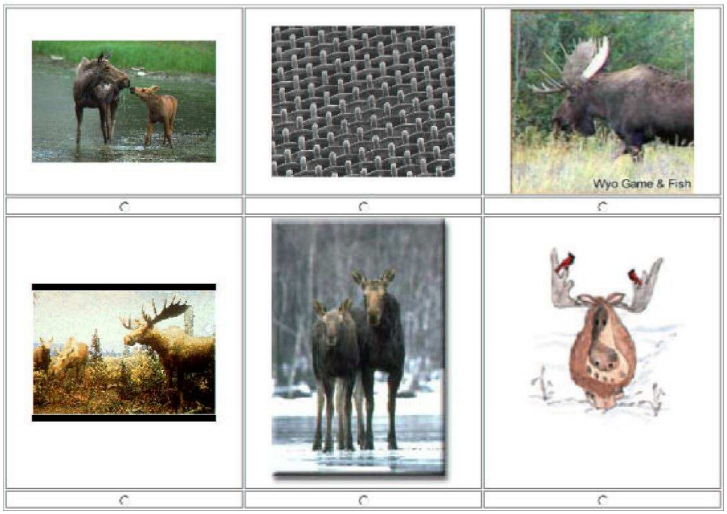
\includegraphics[width=\textwidth]{./img/CAPTCHAtypes/afwijkingCAPTCHA.png}}
         \only<4>{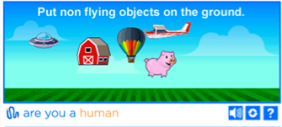
\includegraphics[width=\textwidth]{./img/CAPTCHAtypes/herkenningCAPTCHA.png}}
       \end{center}         
  \end{columns}
\end{frame}
\subsection{Evolutie}
\begin{frame}
  \frametitle{CAPTCHA evolutie}
  \begin{columns}[c]
     \column{.60\textwidth}
       \begin{itemize}
         \item<+-> 1996: Naor beschrijft principe
  	     \item<+-> 2000: Carnegie Mellon Universiteit voor Yahoo
  	     \item<+-> 2008: reCAPTCHA
       \end{itemize}
    \column{.40\textwidth}
      \begin{center}
        \only<2>{
\includegraphics[width=\textwidth]{./img/ez-gimpy.png}}
        \only<3>{
\includegraphics[width=\textwidth]{./img/reCAPTCHA.png}}
      \end{center}
  \end{columns}
\end{frame}
\begin{frame}
  \frametitle{CAPTCHA evolutie}
  \begin{columns}[c]
    \column{.50\textwidth}
       \begin{center}
        \only<1>{
\includegraphics[width=\textwidth]{./img/evolutie/reCAPTCHA2008.png}\\2008}
        \only<1>{
\includegraphics[width=\textwidth]{./img/evolutie/reCAPTCHA2010.png}\\2010}
      \end{center}
     \column{.50\textwidth}
     \begin{center}
        \only<1>{
\includegraphics[width=\textwidth]{./img/evolutie/reCAPTCHA2009.png}\\2009}
        \only<1>{
\includegraphics[width=\textwidth]{./img/evolutie/reCAPTCHA2013.png}\\2013}
      \end{center}
  \end{columns}
\end{frame}
\begin{frame}
  \frametitle{CAPTCHA evolutie - Onmogelijke CAPTCHA}
  Onmogelijke CAPTCHA door verhoogde moeilijkheid
  \begin{columns}[c]
    \column{.50\textwidth}
       \begin{center}
        \only<1>{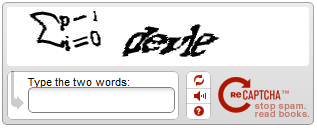
\includegraphics[width=\textwidth]{./img/impos/impossible_captcha01.png}}
      \end{center}
     \column{.50\textwidth}
     \begin{center}
        \only<1>{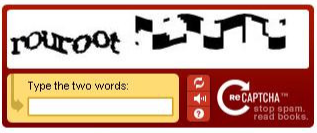
\includegraphics[width=\textwidth]{./img/impos/impossible_captcha04.png}}
      \end{center}
  \end{columns}
\end{frame}
\subsection{Toekomst}
\begin{frame}
  \frametitle{CAPTCHA toekomst}
  \begin{itemize}
    \item<+-> verbetering OCR algoritmen
    \item<+-> toenames in rekenkracht
  \end{itemize}
  \vfill  
  \begin{itemize}
    \item<+-> steeds moeilijkere CAPTCHA
    \item<+-> steeds verbeterende AI
  \end{itemize}
  \onslide<+->{evolutie naar empathie en complexere begrippen}    
\end{frame}
\section{Neurale netwerken}
\subsection{componenten}
\begin{frame}
  \frametitle{neuron componenten}
  \begin{itemize}
    \item<+-> propagatie functie
    \item<+-> drempelwaarde
    \item<+-> activatiefunctie
  \end{itemize}
\end{frame}
\subsection{topologie}
\begin{frame}
  \frametitle{netwerk topologie}
  \begin{itemize}
    \item<+-> feedforward
    \item<+-> recurrent
      \begin{itemize}
        \item direct
        \item indirect
        \item lateraal
      \end{itemize}
    \item<+-> compleet gelinkt
  \end{itemize}
\end{frame}
\begin{frame}
  \frametitle{bias neuron}
  \begin{itemize}
    \item<+-> vervangt de drempelwaarde
    \item<+-> extra neuron per netwerk of laag
    \item<+-> altijd actief
    \item<+-> gewicht is de drempelwaarde
  \end{itemize}
\end{frame}
\subsection{netwerk leren}
\begin{frame}
  \frametitle{leer paradigma}
  \begin{enumerate}
    \item nieuwe connecties
    \item bestaande connecties verwijderen
    \item connectie gewichten aanpassen
    \item drempelwaarden aanpassen
    \item neuron functies aanpassen
    \item nieuwe neuronen aanmaken
    \item bestaande neuronen verwijderen
  \end{enumerate}
\end{frame}
\begin{frame}
  \frametitle{methodes van leren}
  \begin{itemize}
    \item zonder toezicht
    \item versterkend
    \item begeleid
  \end{itemize}
  \vfill
  \begin{itemize}
    \item offline
    \item online
  \end{itemize}
\end{frame}
\part{Implementatie}
\partframe{%
  \vfill%
  
\includegraphics[width=3cm]{logo/HG-woordmerk-inv}%
}
\partTOC
\section{Captcha maker}
\begin{frame}
  \frametitle{CAPTCHA MAKER}
  Dit is gemaakt om het testen van patroon herkenning te vergemakkelijken.
  \begin{itemize}
    \item achtergronden
    \item tekst
    \item ruis
    \item vervormingen
  \end{itemize}
\end{frame}
\section{Neurale netwerken}
\begin{frame}
  \frametitle{Neurale netwerken}
  Met het Encog framework zijn volgende netwerken ge\"{i}mplementeerd
  \begin{itemize}
    \item Hopfield netwerk
    \item perceptron netwerk
    \item Kohonen netwerk
  \end{itemize}
\end{frame}
\begin{frame}
  \frametitle{Hopfield}
  \begin{columns}[c]
     \column{.40\textwidth}
       \begin{itemize}
         \item probleem met capaciteit
       \end{itemize}
     \column{.60\textwidth}
       \only<1>{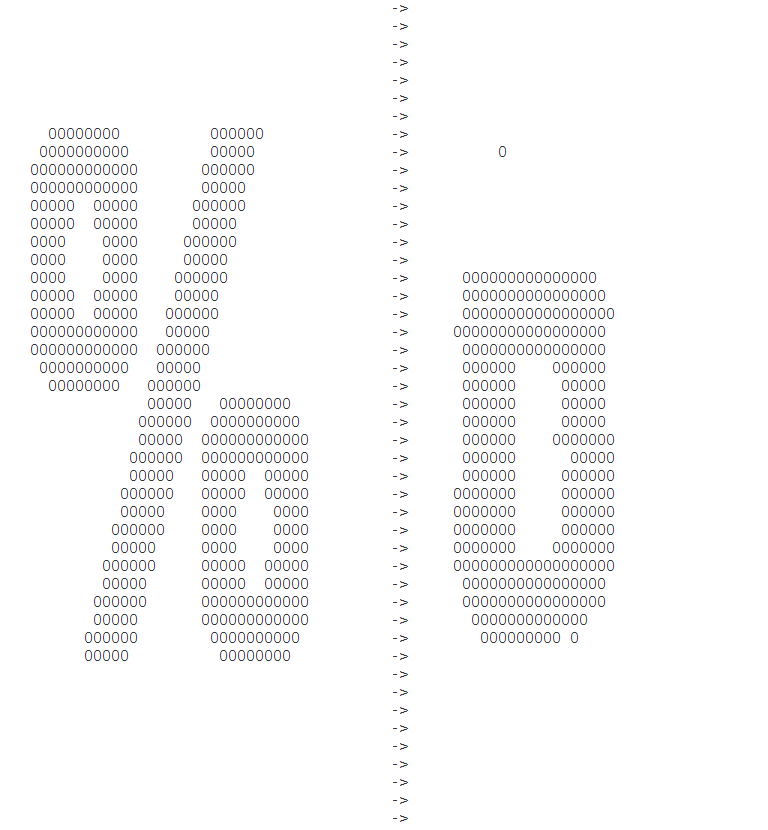
\includegraphics[width=\textwidth]{./img/networks/HopfieldFail.png}}
  \end{columns}
\end{frame}
\begin{frame}
  \frametitle{perceptron}
    \begin{itemize}
      \item netwerk in staat letters te herkennen
      \item batch test optimale configuratie
        \begin{itemize}
          \item maximum 20\% verificatie herkenning
          \item maximum 18\% herkenning bij vervorming
        \end{itemize}
    \end{itemize}
    \vfill
    \only<1>{\rightarrow memorisatie van trainingsset}
\end{frame}
\begin{frame}
  \frametitle{Kohonen}
  Geen succesvol resultaat, foutmarge blijft te hoog
  \vfill
  vermoedelijk knopen tijdens het ontvouwen van het netwerk
\end{frame}
\part{Conclusie}
\partframe{%
  \vfill%
  
\includegraphics[width=3cm]{logo/HG-woordmerk-inv}%
}
\begin{frame}
  \frametitle{Conclusie}
  \begin{itemize}
    \item<+-> CAPTCHA worden steeds moeilijker
    \item<+-> neurale netwerken kunnen patronen herkennen
      \begin{itemize}
        \item<+-> input: verklein en resample
        \item<+-> Hopfield: pseudo-inverse leer regel
        \item<+-> perceptron:
          \begin{itemize}
            \item nauwkeurigheid
            \item lagen
          \end{itemize}
        \item<+-> Kohonen: voorkomen van knopen 
      \end{itemize}
    \item<+-> economische relevantie
  \end{itemize}
\end{frame}
\part{Afronding}
\partframe{%
  \begin{itemize}
    \item Vragen
    \item Bedankt
  \end{itemize}
  \vfill%
  
\includegraphics[width=3cm]{logo/HG-woordmerk-inv}%
}
\begin{frame}{Afronding}
\begin{center}
Vragenronde
\end{center}
\end{frame}
\begin{frame}{Afronding}
\begin{center}
Bedankt voor de aandacht
\end{center}
\end{frame}

%---------- Back matter -------------------------------------------------------

% dia met HoGent logo
\HoGentLogo

\end{document}
